\documentclass[conference]{IEEEtran}
\usepackage{cite,graphicx,booktabs,url}
\usepackage{tikz}
\usetikzlibrary{arrows.meta,positioning,shapes.geometric}
\definecolor{bundleblue}{RGB}{52,101,164}
\definecolor{gateamber}{RGB}{196,160,0}
\definecolor{decisiongreen}{RGB}{78,154,6}

\begin{document}

\title{RelGate: Evidence-Grounded Readiness Gates\\for LLM-Reviewed Cloud Changes}

\author{\IEEEauthorblockN{Lokesh Chauhan}
\IEEEauthorblockA{Independent Researcher\\
Dallas, TX, USA\\
lokesh0186@gmail.com}}

\maketitle

\renewcommand{\thefootnote}{\fnsymbol{footnote}}
\footnotetext[1]{This work was conducted independently and does not relate to the author's employment. No employer resources, data, or confidential information were used.}
\renewcommand{\thefootnote}{\arabic{footnote}}

\begin{abstract}
Pre-deployment review of cloud changes is a reliability activity: reviewers must decide whether a change has enough evidence for observability, alerting, rollout safety, rollback, ownership, reliability impact, and validation.
Large language models can assist this review, but free-form answers may be poorly calibrated.
They can either approve unsupported changes or block changes that already contain sufficient readiness evidence.
We present RelGate, a project prototype and experimental framework that requires LLM-generated readiness decisions to cite exact evidence from the change bundle or mark the evidence as missing.
In a 12-scenario pilot across three models and three review modes (108 calls), all modes avoided false-ready approvals on unsafe changes, but free-form review blocked all READY controls.
RelGate achieved the best calibration in this pilot, with zero observed false-ready decisions, zero observed false-blocks, and fewer unsupported evidence claims than checklist-only review (0.053 vs.\ 0.208).
These early results suggest that evidence-grounded review may improve the auditability and release precision of LLM-assisted production-readiness gates.
\end{abstract}

\section{Motivation}

Cloud services deploy many changes daily, each requiring production-readiness evidence for safe release~\cite{beyer2016sre}.
Consider a scenario in which a change bundle includes explicit dashboard links, alert rules, a staged rollout plan, a rollback trigger, on-call ownership, SLO-impact analysis, and validation test results.
In our pilot, free-form LLM review returned FIX-BEFORE-SHIP for such a fully-specified change across all three tested models, typically requesting generic additional assurance despite all evidence being present.
Conversely, giving the same models a structured checklist produced correct READY decisions in most cases, but sometimes marked gates as satisfied without citing supporting text from the bundle.

The pilot exposes a calibration problem: free-form review can be safe but over-conservative, while checklist review can improve decisions yet encourage unsupported completion.
More broadly, unsupported readiness claims create a false sense of auditability, where the gate says ``pass'' but the supporting evidence is fabricated or paraphrased rather than cited~\cite{huang2023hallucination}.
As LLM-assisted review enters production workflows~\cite{yan2025empirical}, this calibration gap becomes a reliability concern.
RelGate addresses it by requiring exact evidence citations for every passing gate, treating readiness review as an auditable evidence-checking problem rather than a free-form advisory task.

\section{RelGate Design}

\begin{figure}[t]
\centering
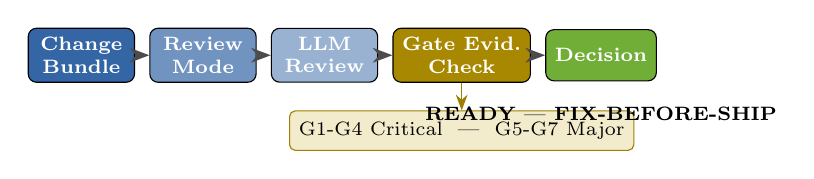
\begin{tikzpicture}[
  node distance=0.45cm and 0.18cm,
  box/.style={draw, rounded corners=3pt, minimum height=0.65cm, minimum width=1.35cm, font=\scriptsize\bfseries, align=center, text=white},
  gate/.style={draw, rounded corners=2pt, minimum height=0.5cm, minimum width=1.7cm, font=\scriptsize, fill=gateamber!20, draw=gateamber!80!black, align=center},
  decision/.style={draw, rounded corners=3pt, minimum height=0.65cm, minimum width=1.2cm, font=\scriptsize\bfseries, align=center, fill=decisiongreen!80, text=white},
  arr/.style={-{Stealth[length=2.5mm]}, thick, color=black!70},
]
\node[box, fill=bundleblue] (bundle) {Change\\Bundle};
\node[box, fill=bundleblue!70, right=of bundle] (mode) {Review\\Mode};
\node[box, fill=bundleblue!50, right=of mode] (llm) {LLM\\Review};
\node[box, fill=gateamber!85!black, right=of llm] (gates) {Gate Evid.\\Check};
\node[decision, right=of gates] (dec) {Decision};

\draw[arr] (bundle) -- (mode);
\draw[arr] (mode) -- (llm);
\draw[arr] (llm) -- (gates);
\draw[arr] (gates) -- (dec);

\node[gate, below=0.35cm of gates] (glist) {G1-G4 Critical~~|~~G5-G7 Major};

\draw[-{Stealth[length=2mm]}, color=gateamber!80!black] (gates) -- (glist);

\node[font=\scriptsize, below=0.2cm of dec] (out) {\textbf{READY} | \textbf{FIX-BEFORE-SHIP}};
\end{tikzpicture}
\caption{RelGate workflow. The model evaluates a change bundle against seven readiness gates and must cite exact evidence for each passing gate; missing evidence produces a FIX-BEFORE-SHIP decision.}
\label{fig:arch}
\end{figure}

RelGate evaluates cloud changes against seven production-readiness gates: \textbf{G1}~Observability (dashboard/metric/log evidence), \textbf{G2}~Alerting (failure-mode coverage), \textbf{G3}~Rollout Safety (staged deployment or blast-radius control), \textbf{G4}~Rollback (revert plan with trigger), \textbf{G5}~Ownership (on-call and escalation), \textbf{G6}~Reliability Impact (SLO or error-budget analysis), and \textbf{G7}~Validation (test/staging evidence).
Gates G1-G4 are critical: if any critical gate lacks cited evidence, the decision must be FIX-BEFORE-SHIP.
Gates G5-G7 are major: missing evidence triggers a warning but does not block.

The \emph{evidence-grounding rule} requires the model to cite exact text from the change bundle for each PASS verdict. If no supporting text exists, the model must report MISSING\_EVIDENCE and recommend a specific remediation. The model must not infer or fabricate evidence. This changes the review task from checklist completion to evidence auditing.

\section{Pilot Study}

We constructed 12 change scenarios: 9 with seeded reliability gaps (missing alerts, absent rollback plans, vague ownership) and 3 READY controls with complete evidence for all seven gates.
Each scenario was evaluated under three prompting modes:
\textbf{M0 Freeform} (unstructured review request),
\textbf{M1 Checklist} (G1-G7 listed; pass/fail per gate),
and \textbf{M2 Evidence-Grounded} (G1-G7 plus the evidence-grounding rule).
Three models were used via OpenRouter at temperature~0: GPT-5.5, Grok~4.3, and Llama~4~Maverick.
This yields 12 x 3 x 3 = 108 evaluation calls.
The artifact contains the scenario schema, prompts, raw outputs, scoring script, and summary metrics.

\textbf{Metrics.}
We report Critical Gap Recall (fraction of seeded critical gaps identified), False-Ready Rate (unsafe changes approved, $n{=}27$ per mode), False-Block Rate (safe controls blocked, $n{=}9$ per mode), Unsupported Evidence Claims (the fraction of explicit readiness-evidence claims not directly supported by the scenario text), Decision Accuracy ($n{=}36$ per mode), and Actionability (0-2 specificity scale).

\section{Preliminary Results}

\begin{table}[t]
\centering
\caption{Pilot results across review modes (averaged over 3 models, 12 cases each).}
\label{tab:results}
\footnotesize
\begin{tabular}{@{}lccc@{}}
\toprule
\textbf{Metric} & \textbf{M0} & \textbf{M1} & \textbf{M2} \\
\midrule
Critical Gap Recall & 0.975 & 1.000 & 1.000 \\
False-Ready Rate ($n{=}27$) & 0.000 & 0.000 & 0.000 \\
False-Block Rate ($n{=}9$) & 1.000 & 0.111 & 0.000 \\
Unsupported Evid.\ Claims & 0.062 & 0.208 & 0.053 \\
Decision Accuracy ($n{=}36$) & 0.750 & 0.972 & 1.000 \\
Actionability (0-2) & 1.58 & 1.74 & 1.74 \\
\bottomrule
\end{tabular}
\end{table}

Table~\ref{tab:results} summarizes results.
We observe three findings:

\textbf{(1) Free-form review is safe but over-conservative.}
M0 detected nearly all seeded gaps (0.975 critical recall) but blocked every change, including all READY controls (false-block = 1.000), yielding 0.750 decision accuracy.

\textbf{(2) Checklist structure improved specificity but increased unsupported claims.}
M1 reduced false-block to 0.111 and reached 0.972 accuracy.
However, its unsupported-evidence rate (0.208) was about four times higher than M2.
The checklist structure encouraged models to mark gates as satisfied by paraphrasing text rather than citing verbatim evidence.

\textbf{(3) Evidence grounding improved calibration by allowing READY controls while preserving zero observed false-ready approvals.}
M2 achieved 1.000 decision accuracy with no false-ready and no false-block.
The evidence-grounding rule forced models to cite real bundle text or honestly report missing evidence, yielding the lowest unsupported-claim rate (0.053).

The main lesson is that production-readiness review should be evaluated as an evidence-auditing task, not only as a pass/fail classification task.

\textbf{Qualitative example.}
On READY control C10 (a Kubernetes HPA addition with full evidence), all three free-form reviews returned FIX-BEFORE-SHIP despite complete readiness evidence.
RelGate approved the same case by citing the rollout plan, rollback trigger, alert rule, dashboard, owner, SLO statement, and load-test results.
In one M1 review of C08 (a queue-worker change with empty alerting), Grok~4.3 quoted a paraphrased rollback plan as evidence, illustrating unsupported completion.

\section{Discussion and Limitations}

\textbf{Relevance to ISSRE.}
RelGate is intended as a discussion-starting project artifact: a small benchmark, prompt family, and scoring rubric for studying calibrated LLM-assisted change review.
Production-readiness review is a reliability activity where missed gaps cause incidents and excessive blocking delays safe releases~\cite{beyer2016sre,gunawi2016bugs}.
As cloud services increasingly adopt LLM-assisted workflows~\cite{yan2025empirical}, calibration and auditability of automated gates become reliability concerns that ISSRE is well-positioned to address.

\textbf{Limitations.}
This pilot uses 12 synthetic scenarios; real production changes exhibit greater diversity and ambiguity.
READY controls are fully specified; real readiness evidence may be ambiguous, stale, or organization-specific.
Evidence presence does not guarantee actual production safety; it only makes the decision auditable against the provided bundle.
Model versions evolve rapidly; results with GPT-5.5, Grok~4.3, and Llama~4~Maverick may not generalize.
We have not yet measured latency, cost, or developer trust in deployment.

\textbf{Next steps.}
We plan to expand to 50+ scenarios from anonymized change records, conduct a developer study, and integrate RelGate into a CI/CD pipeline~\cite{ahmed2023recommending}.

\textbf{Artifact:} \url{https://github.com/lokesh0186/relgate}

\bibliographystyle{IEEEtran}
\bibliography{references}

\end{document}
